% https://habrahabr.ru/post/145523/
% http://fsweb.info/editors/latex/presentation.html
\documentclass[10pt]{beamer}
\usepackage[utf8]{inputenc}
\usepackage[T2A]{fontenc}
\usepackage[english, russian]{babel}
\usepackage{amsmath,amsfonts,amssymb}
\usepackage{graphicx}
%\usetheme{Singapore}
% \usetheme{Berlin}
% \usetheme{CambridgeUS}
\usetheme{CambridgeUS}

%\setbeamercolor{элемент}{bg=цвет1,fg=цвет2}. Здесь «элемент» — название элемента, чей цвет мы хотим изменить (например, «normal text» — обычный текст), «bg» — цвет фона, «fg» — цвет текста.
%\usebackgroundtemplate{\includegraphics[width=\paperwidth,height=\paperheight]{my_backgroung_picture.jpg}}

\addto\captionsrussian{\renewcommand{\figurename}{Рис.}}
\setbeamertemplate{caption}[numbered]

\RequirePackage{caption}
\DeclareCaptionLabelSeparator{defffis}{ -- }
\captionsetup{justification=centering,labelsep=defffis}

\newcommand{\MB}{\mathbf}
\newcounter{myexmpl}



\begin{document}


\title{Эргономика компьютерных игр}
\subtitle{презентация по курсу ``Человеко-компьютерное взаимодействие''}
\author{В.Э. Смирнов, Д.В. Сухоловский}
\institute{ЮФУ, каф. МОП ЭВМ}
\date{2017 год
\vspace{10mm}

\centering

\includegraphics[scale=0.25]{res/img/titlePage/sfedu.png}
}
\setbeamercovered{transparent}
% Если в нашей презентации используется последовательное высвечивание элементов, стоит сказать: \setbeamercovered{transparent}, чтобы неактивные элементы были хотя бы немного видны.

%\setbeamertemplate{navigation symbols}{}  %убрать панель навигации

%	\author{}
	%\title{}
	%\subtitle{}
	%\logo{}
	%\institute{}
	%\date{}
	%\subject{}
	%\setbeamercovered{transparent} % или dynamic
	%\setbeamertemplate{navigation symbols}{}


%%%%%%%%%%%%%%%%%%% титул - слайд 1  %%%%%%%%%%%%%%%%%%%%%%
\begin{frame}[plain]
	%\maketitle
  \titlepage
\end{frame}

%%%%%%%%%%%%%%%%%%%%%%%% содержание - слайд 2 %%%%%%%%%%%%%%%%%%%%%%%%%%%%%%%%

\begin{frame}
  \frametitle{Содержание}
  \tableofcontents
\end{frame}

%%%%%%%%%%%%%%%%%%%%%%%%%%%%%%%%%%%%%%%%%%%%%%%%%%%%%%%%%%%%%%%%%%%%%
\section{Возможности Visual Studio}
% \subsection{Особенности СТУ}

%%%%%%%%%%%%%%%%%%%%%%%%%%  слайд 3 %%%%%%%%%%%%%%%%%%%%%%%%%%%%

\begin{frame}[shrink=8]
\frametitle{Качество ПО}

\begin{columns}[c]
\column{0.5\textwidth}

\begin{center}
  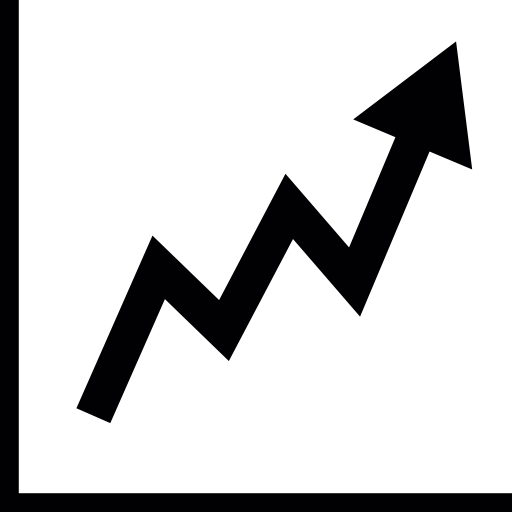
\includegraphics[width=0.8\textwidth]{res/img/improve.png}
  Улучшение
\end{center}

\column{0.5\textwidth}
\begin{block}{}
\begin{itemize}
  \item Качество программ -- понятие, аккумулирующее противоречия природы самих программ и противоречия, возникающие при их создании
  \item Профилирование -- сбор характеристик работы программы
  \item Оптимизация -- модификация программы для улучшения её эффективности
\end{itemize}
\end{block}

\end{columns}


\end{frame}

%%%%%%%%%%%%%%%%%%%%%%%%%%  слайд 4 %%%%%%%%%%%%%%%%%%%%%%%%%%%%
\begin{frame}%[label=main_descr_0]
\frametitle{Профилирование в Visual Studio}

\begin{columns}[c]
\column{0.5\textwidth}

\begin{center}
  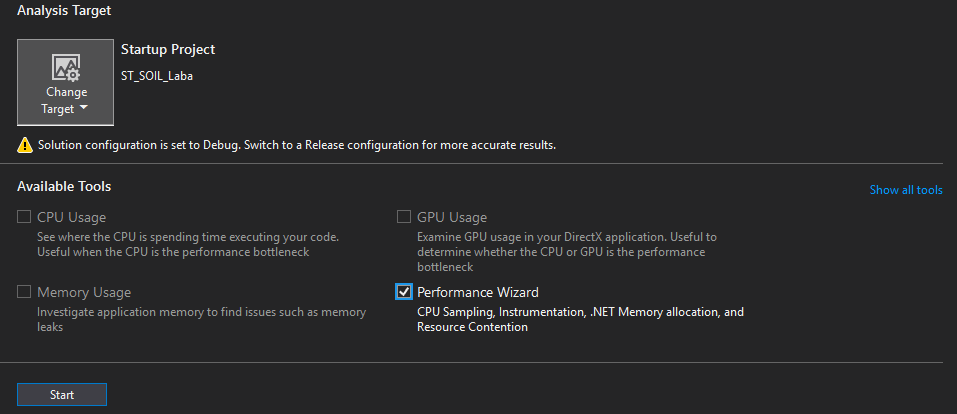
\includegraphics[width=\textwidth]{res/img/AnalysisTarget.png}
  Режимы работы профайлера
\end{center}

\column{0.5\textwidth}
\begin{block}{}
\begin{itemize}
  \item Visual Studio имеет возможности для профилирования:
  \begin{itemize}
    \item Использования процессора (CPU Usage)
    \item Использования видеокарты (GPU Usage)
    \item Использования памяти (Memory Usage)
    \item Общей производительности (Performance Wizard)
  \end{itemize}
\end{itemize}
\end{block}

\end{columns}

\end{frame}

%%%%%%%%%%%%%%%%%%%%%%%%%%  слайд 5 %%%%%%%%%%%%%%%%%%%%%%%%%%%%

\begin{frame}%[shrink=20,fragile]
\frametitle{Performance Wizard}

\begin{columns}[c]
\column{0.5\textwidth}

\begin{center}
  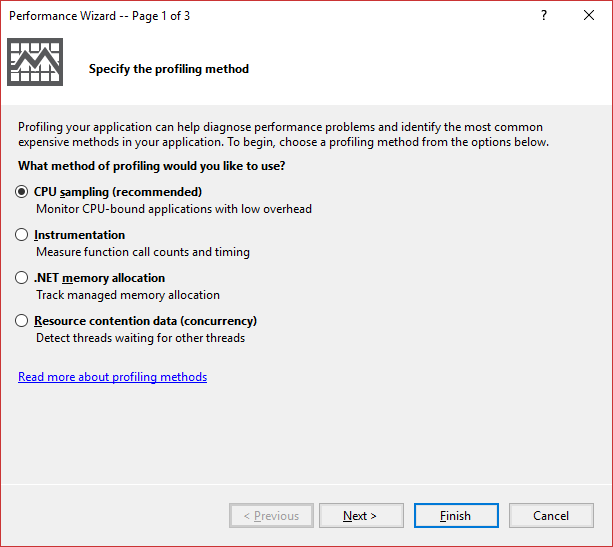
\includegraphics[width=\textwidth]{res/img/AnalysisTargetWizard.png}
  Параметры Performance Wizard
\end{center}

\column{0.5\textwidth}
\begin{block}{}
\begin{itemize}
  \item При выборе Performance Wizard можно дополнительно выбрать параметры для профилирования
  \item Из предложенных далее будет использоваться только CPU sampling
\end{itemize}
\end{block}

\end{columns}

\end{frame}

%%%%%%%%%%%%%%%%%%%%%%%%%%%%%%%%%  слайд 6 %%%%%%%%%%%%%%%%%%%%%%%%%%%%%%%%%%%%%%%%%%%%%%5

\section{Исходная программа}


\begin{frame}%[label=main_descr_1]
\frametitle{Исходная программа}


\begin{block}

\begin{itemize}
\item Программа генерирует изображение, на котором изображено
\begin{itemize}
  \item N точек разного цвета
\end{itemize}
\item Положение и цвет точек может задаваться
\begin{itemize}
  \item Пользователем
  \item Случайным образом
\end{itemize}
\item Остальные области изображение закрашиваются цветом, противоположным той точке, к которой они ближе всего находятся
\end{itemize}

\end{block}

\end{frame}


%%%%%%%%%%%%%%%%%%%%%%%%%%%%%%%%%  слайд 7 %%%%%%%%%%%%%%%%%%%%%%%%%%%%%%%%%%%%%%%%%%%%%%5

\section{Анализ программы}


\begin{frame}
\frametitle{Диаграмма Вороного}


\begin{columns}[c]
\column{0.5\textwidth}

\begin{center}
  
\includegraphics[width=\textwidth]{res/img/VoronoiDiagram.png}
  Результат работы программы
\end{center}

\column{0.5\textwidth}
\begin{block}{}
\begin{itemize}
  \item Такое разбиение плоскости (в данном случае изображения) называется диаграммой Вороного
  \item Результатом работы программы является изображение, которое разделено на 32 области
\end{itemize}
\end{block}

\end{columns}

\end{frame}

%%%%%%%%%%%%%%%%%%%%%%%%%  слайд 8 %%%%%%%%%%%%%%%%%%%%%%%%%%
\begin{frame}
\frametitle{Первичная оценка программы}


\begin{columns}[c]
\column{0.5\textwidth}

\begin{center}
  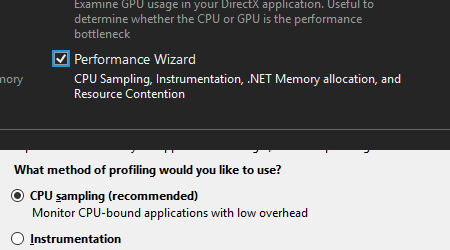
\includegraphics[width=\textwidth]{res/img/AnalysisTargetWay.png}
  Выбор режима профилирования
\end{center}

\column{0.5\textwidth}
\begin{block}{}
\begin{itemize}
  \item Тля того, чтобы знать откуда начать и куда двигаться, стоит сначала сделать первичную оценку того состояния, в котором находится программу
  \item Для этого можно запустить анализ в Performance Wizard
\end{itemize}
\end{block}

\end{columns}

\end{frame}


%%%%%%%%%%%%%%%%%%%%%%%%%  слайд 9 %%%%%%%%%%%%%%%%%%%%%%%%%%
\begin{frame}
\frametitle{Результаты первичного анализа}


\begin{columns}[c]
\column{0.5\textwidth}

\begin{center}
  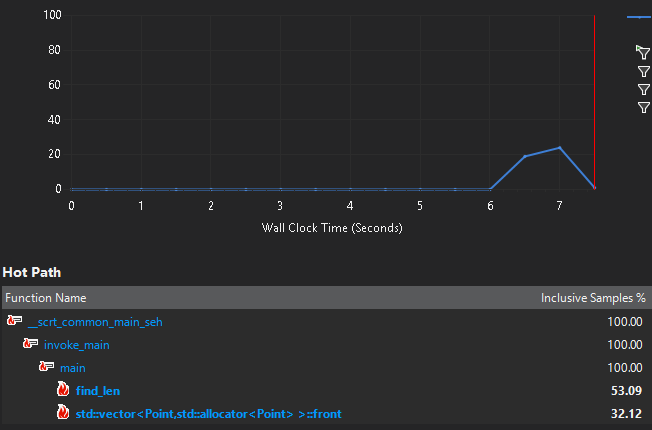
\includegraphics[width=\textwidth]{res/img/AnalysisTargetWizard1SummaryCropped.png}
  График выполнения программы
\end{center}

\column{0.5\textwidth}
\begin{block}{}
  \begin{itemize}
    \item По результатам анализа видно, что основное процессорное время берут
    \begin{itemize}
      \item vector::begin() -- 32.1\%
      \item find\_len() -- 53.1\%
    \end{itemize}
  \end{itemize}
\end{block}

\end{columns}

\end{frame}


%%%%%%%%%%%%%%%%%%%%%%%%%  слайд 10 %%%%%%%%%%%%%%%%%%%%%%%%%%
\begin{frame}
\frametitle{Результаты первичного анализа. Взгляд на код}


\begin{columns}[c]
\column{0.5\textwidth}

\begin{center}
  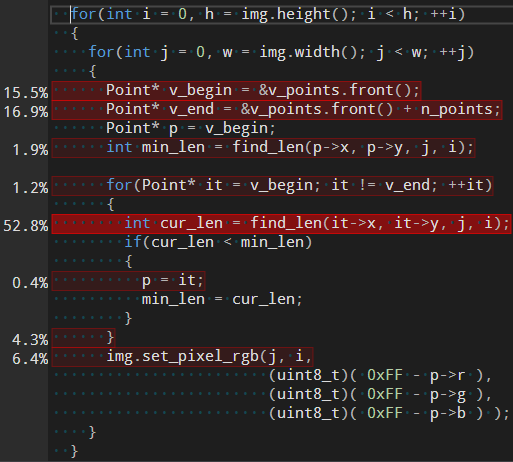
\includegraphics[width=\textwidth]{res/img/AnalysisTargetWizard1CodeCropped.png}
  Исходный код места проблемы
\end{center}

\column{0.5\textwidth}
\begin{block}{}
  \begin{itemize}
    \item Тот факт, что метод vector::begin() брал на себя столько процессорного времени был неожиданностью
    \item Функция find\_len() отбирает наибольшую часть процессорного времени, поэтому ее тоже стоит рассмотреть
  \end{itemize}
\end{block}

\end{columns}

\end{frame}


%%%%%%%%%%%%%%%%%%%%%%%%%  слайд 11 %%%%%%%%%%%%%%%%%%%%%%%%%%

\section{Модификация программы}


\begin{frame}
\frametitle{Улучшение 1}


\begin{columns}[c]
\column{0.5\textwidth}

\begin{center}
  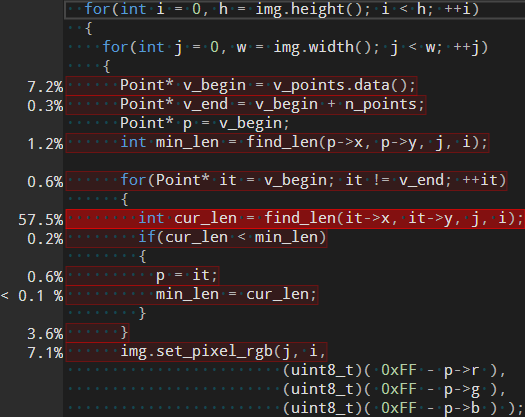
\includegraphics[width=\textwidth]{res/img/AnalysisTargetWizard2CodeCropped.png}
  Улучшение
\end{center}

\column{0.5\textwidth}
\begin{block}{}
  \begin{itemize}
    \item Замена метода vector::begin() на vector::data()
    \item Переиспользование ранее определенных переменных вместо вызова метода повторно
  \end{itemize}
\end{block}

\end{columns}

\end{frame}


%%%%%%%%%%%%%%%%%%%%%%%%%  слайд 12 %%%%%%%%%%%%%%%%%%%%%%%%%%
\begin{frame}
\frametitle{Проблемы и варианты решений}


\begin{block}{}
  \begin{itemize}
    \item Неоптимальный алгоритм
    \begin{itemize}
      \item Изменить алгоритм построения диаграммы Вороного
    \end{itemize}
    \item Чрезмерное использование функции find\_len()
    \begin{itemize}
      \item Заранее просчитать все возможные значения функции, а в дальнейшем обращаться лишь к двумерному массиву
    \end{itemize}
    \item Однопоточная программа
    \begin{itemize}
      \item Распараллелить алгоритм на все ядра процессора
    \end{itemize}
  \end{itemize}
\end{block}


\end{frame}


%%%%%%%%%%%%%%%%%%%%%%%%%  слайд 13 %%%%%%%%%%%%%%%%%%%%%%%%%%
\begin{frame}
\frametitle{Кэширование результатов функции find\_len()}


\begin{columns}[c]
\column{0.5\textwidth}

\begin{center}
  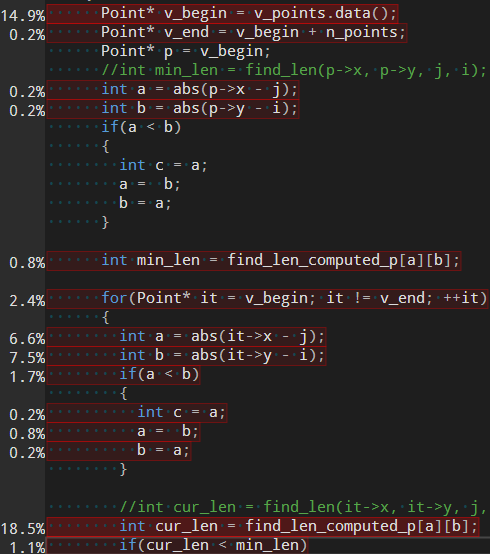
\includegraphics[width=\textwidth]{res/img/AnalysisTargetWizard3CodeCropped.png}
  Код рассматриваемого места
\end{center}

\column{0.5\textwidth}
\begin{block}{}
  \begin{itemize}
    \item Дальнейшее улучшение программы будет двигаться в сторону кэширования из за того что
    \begin{itemize}
      \item Функция find\_len() находится внутри 3-х уровневого цикла
      \item Очень много вызовов функции с одними и теми же параметрами
      \item Другие алгоритмы сложны в реализации
  \end{itemize}
  \end{itemize}
\end{block}

\end{columns}

\end{frame}


%%%%%%%%%%%%%%%%%%%%%%%%%  слайд 14 %%%%%%%%%%%%%%%%%%%%%%%%%%
\begin{frame}
\frametitle{Улучшение 2}


\begin{columns}[c]
\column{0.5\textwidth}

\begin{center}
  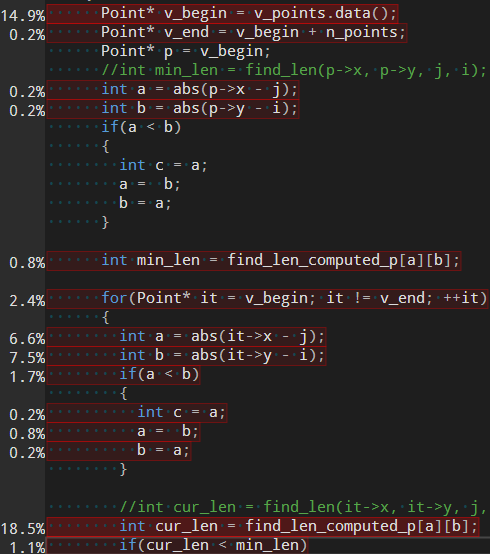
\includegraphics[width=\textwidth]{res/img/AnalysisTargetWizard3CodeCropped.png}
  Улучшенный код
\end{center}

\column{0.5\textwidth}
\begin{block}{}
  \begin{itemize}
    \item Перед выполнением 3-х уровневого цикла были
    \begin{itemize}
      \item Закэшированы все возможные значения функции find\_len()
      \item Добавлены оптимизации по уменьшению использования памяти
    \end{itemize}
    \item Внутри цикла
    \begin{itemize}
      \item Обращение к функции заменено на обращение к массиву
    \end{itemize}
  \end{itemize}
\end{block}

\end{columns}

\end{frame}


%%%%%%%%%%%%%%%%%%%%%%%%%  слайд 15 %%%%%%%%%%%%%%%%%%%%%%%%%%
\begin{frame}
\frametitle{Анализ изменений}


\begin{columns}[c]
\column{0.5\textwidth}

\begin{center}
  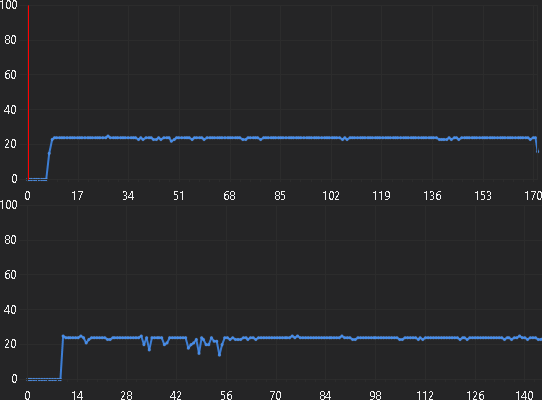
\includegraphics[width=\textwidth]{res/img/AnalysisTargetWizardTestCropped.png}
  Графики выполнения. До и после
\end{center}

\column{0.5\textwidth}
\begin{block}{}
  \begin{itemize}
    \item С одинаковыми параметрами на входе программы она отработала
    \begin{itemize}
      \item На 28 секунд быстрее
      \item Примерно на 15\% быстрее памяти
    \end{itemize}
    \item При определенных условиях относительный прирост может быть больше
  \end{itemize}
\end{block}

\end{columns}

\end{frame}


%%%%%%%%%%%%%%%%%%%%%%%%%  слайд 16 %%%%%%%%%%%%%%%%%%%%%%%%%%
\begin{frame}
\frametitle{Заключение}


\begin{block}{}
  \begin{itemize}
    \item Visual Studio представляет собой мощное средство для разработки ПО которое включает в себя очень много различных инструментов
    \item Используя возможности профилирования, в программе были найдены места, нуждающиеся в оптимизации, которые были улучшены
    \item Дополнительно к проделанной работе можно распараллелить программу, что даст значительный прирост, если компьютер имеет больше одного ядра процессора
    \item Проделанные улучшения не являются единственно верными. Кроме них можно провести так же другие улучшения, которое, возможно, приведут к лучшему результату
  \end{itemize}
\end{block}


\end{frame}



\end{document}
